%% Manuscript for Computer Methods and Programs in Biomedicine (Elsevier, elsarticle class).
%% Build:  tectonic main.tex      (all numbers come from numbers.tex, generated by make_numbers_tex.py)
\documentclass[preprint,review,12pt]{elsarticle}

\usepackage{amsmath,amssymb,bm}
\usepackage{booktabs}
\usepackage{xcolor}
\usepackage{lineno}
\usepackage[hidelinks]{hyperref}
\linenumbers

% AUTO-GENERATED by make_numbers_tex.py --mode fp32 -- do not edit by hand
\newcommand{\NSiamSeeds}{3}
\newcommand{\NBOneSeeds}{3}
\newcommand{\InferenceMode}{full-precision (fp32), deterministic}
\newcommand{\SiamClosedAcc}{94.79 $\pm$ 0.21}
\newcommand{\SiamClosedAccMean}{94.79}
\newcommand{\SiamClosedFOne}{0.943 $\pm$ 0.004}
\newcommand{\SiamClosedFOneMean}{0.943}
\newcommand{\BOneClosedAcc}{93.91 $\pm$ 0.54}
\newcommand{\BOneClosedAccMean}{93.91}
\newcommand{\BOneClosedFOne}{0.930 $\pm$ 0.007}
\newcommand{\BOneClosedFOneMean}{0.930}
\newcommand{\SiamClosedSens}{0.946 $\pm$ 0.003}
\newcommand{\SiamClosedSensMean}{0.946}
\newcommand{\SiamClosedPrec}{0.944 $\pm$ 0.005}
\newcommand{\SiamClosedPrecMean}{0.944}
\newcommand{\SiamClosedSpec}{0.9958 $\pm$ 0.0001}
\newcommand{\SiamClosedSpecMean}{0.9958}
\newcommand{\SiamHeadClosedAcc}{95.72 $\pm$ 0.35}
\newcommand{\SiamHeadClosedAccMean}{95.72}
\newcommand{\CmpFeatDiff}{+0.47}
\newcommand{\CmpFeatCI}{[-1.21, +2.04]}
\newcommand{\CmpFeatFOneDiff}{+0.006}
\newcommand{\CmpFeatFOneCI}{[-0.010, +0.031]}
\newcommand{\CmpFeatMcN}{48 vs 39}
\newcommand{\CmpFeatMcP}{0.39}
\newcommand{\CmpHeadDiff}{+1.37}
\newcommand{\CmpHeadCI}{[-0.38, +3.06]}
\newcommand{\CmpHeadFOneDiff}{+0.014}
\newcommand{\CmpHeadFOneCI}{[-0.002, +0.039]}
\newcommand{\CmpHeadMcN}{54 vs 28}
\newcommand{\CmpHeadMcP}{0.0054}
\newcommand{\CmpGfslDiff}{+1.99}
\newcommand{\CmpGfslCI}{[-0.54, +4.72]}
\newcommand{\CmpGfslFOneDiff}{+0.017}
\newcommand{\CmpGfslFOneCI}{[-0.007, +0.044]}
\newcommand{\CmpGfslMcN}{90 vs 49}
\newcommand{\CmpGfslMcP}{0.00064}
\newcommand{\SeedClosedRange}{+0.05 to +1.47}
\newcommand{\SeedClosedNPos}{9}
\newcommand{\SeedClosedNSig}{0}
\newcommand{\SeedClosedN}{9}
\newcommand{\SeedClosedFOneRange}{+0.000 to +0.021}
\newcommand{\SeedClosedFOneNSig}{1}
\newcommand{\SeedNcmRange}{+1.36 to +2.72}
\newcommand{\SeedNcmNPos}{9}
\newcommand{\SeedNcmNSig}{2}
\newcommand{\SeedNcmN}{9}
\newcommand{\SeedNcmFOneRange}{-0.014 to +0.017}
\newcommand{\SeedNcmFOneNSig}{0}
\newcommand{\SiamGfslAcc}{89.56 $\pm$ 0.36}
\newcommand{\SiamGfslAccMean}{89.56}
\newcommand{\SiamGfslFOne}{0.786 $\pm$ 0.008}
\newcommand{\SiamGfslFOneMean}{0.786}
\newcommand{\SiamGfslRare}{74.5 $\pm$ 2.7}
\newcommand{\SiamGfslRareMean}{74.5}
\newcommand{\BOneGfslFOne}{0.785 $\pm$ 0.008}
\newcommand{\BOneGfslFOneMean}{0.785}
\newcommand{\BOneGfslAcc}{87.57 $\pm$ 0.38}
\newcommand{\BOneGfslAccMean}{87.57}
\newcommand{\BOneGfslRare}{77.4 $\pm$ 1.7}
\newcommand{\BOneGfslRareMean}{77.4}
\newcommand{\SiamGfslBase}{91.8 $\pm$ 0.3}
\newcommand{\SiamGfslBaseMean}{91.8}
\newcommand{\BOneGfslBase}{89.4 $\pm$ 0.6}
\newcommand{\BOneGfslBaseMean}{89.4}
\newcommand{\HeadRareMin}{33}
\newcommand{\HeadRareMax}{43}
\newcommand{\CeAcc}{93.10}
\newcommand{\CeFOne}{0.897}
\newcommand{\DengueToSapMin}{32}
\newcommand{\DengueToSapMax}{35}
\newcommand{\DengueTest}{44}
\newcommand{\KshotSiamOne}{37.3 $\pm$ 2.3}
\newcommand{\KshotSiamOneMean}{37.3}
\newcommand{\KshotBOneOne}{30.8 $\pm$ 2.4}
\newcommand{\KshotBOneOneMean}{30.8}
\newcommand{\KshotSiamFive}{64.6 $\pm$ 1.2}
\newcommand{\KshotSiamFiveMean}{64.6}
\newcommand{\KshotBOneFive}{67.9 $\pm$ 1.8}
\newcommand{\KshotBOneFiveMean}{67.9}
\newcommand{\KshotDraws}{100}
\newcommand{\NGfslSiam}{3}
\newcommand{\NGfslBOne}{3}
\newcommand{\LrWinsN}{6}
\newcommand{\NCheckpoints}{7}
\newcommand{\LrWinExceptions}{baseline seed 1 (shrunk Mahalanobis classifier)}
\newcommand{\WinSiamLr}{3}
\newcommand{\WinBOneLr}{2}
\newcommand{\WinSiamMaha}{0}
\newcommand{\WinBOneMaha}{1}
\newcommand{\WinSiamNcm}{0}
\newcommand{\WinBOneNcm}{0}
\newcommand{\WinSiamDc}{0}
\newcommand{\WinBOneDc}{0}
\newcommand{\SiamNcmFOne}{0.786 $\pm$ 0.008}
\newcommand{\SiamNcmFOneMean}{0.786}
\newcommand{\SiamNcmAcc}{89.56 $\pm$ 0.36}
\newcommand{\SiamNcmAccMean}{89.56}
\newcommand{\SiamNcmBase}{91.8 $\pm$ 0.3}
\newcommand{\SiamNcmBaseMean}{91.8}
\newcommand{\SiamNcmKOne}{36.9 $\pm$ 2.6}
\newcommand{\SiamNcmKOneMean}{36.9}
\newcommand{\BOneNcmFOne}{0.785 $\pm$ 0.008}
\newcommand{\BOneNcmFOneMean}{0.785}
\newcommand{\BOneNcmKOne}{29.7 $\pm$ 2.0}
\newcommand{\BOneNcmKOneMean}{29.7}
\newcommand{\SiamLrFOne}{0.849 $\pm$ 0.009}
\newcommand{\SiamLrFOneMean}{0.849}
\newcommand{\SiamLrAcc}{92.72 $\pm$ 0.27}
\newcommand{\SiamLrAccMean}{92.72}
\newcommand{\SiamLrBase}{94.6 $\pm$ 0.1}
\newcommand{\SiamLrBaseMean}{94.6}
\newcommand{\SiamLrKOne}{18.0 $\pm$ 0.8}
\newcommand{\SiamLrKOneMean}{18.0}
\newcommand{\BOneLrFOne}{0.855 $\pm$ 0.013}
\newcommand{\BOneLrFOneMean}{0.855}
\newcommand{\BOneLrKOne}{14.6 $\pm$ 1.4}
\newcommand{\BOneLrKOneMean}{14.6}
\newcommand{\SiamMahaFOne}{0.861 $\pm$ 0.008}
\newcommand{\SiamMahaFOneMean}{0.861}
\newcommand{\SiamMahaAcc}{92.56 $\pm$ 0.69}
\newcommand{\SiamMahaAccMean}{92.56}
\newcommand{\SiamMahaBase}{94.4 $\pm$ 0.9}
\newcommand{\SiamMahaBaseMean}{94.4}
\newcommand{\SiamMahaKOne}{25.3 $\pm$ 4.8}
\newcommand{\SiamMahaKOneMean}{25.3}
\newcommand{\BOneMahaFOne}{0.846 $\pm$ 0.001}
\newcommand{\BOneMahaFOneMean}{0.846}
\newcommand{\BOneMahaKOne}{15.5 $\pm$ 1.2}
\newcommand{\BOneMahaKOneMean}{15.5}
\newcommand{\SiamDcFOne}{0.776 $\pm$ 0.008}
\newcommand{\SiamDcFOneMean}{0.776}
\newcommand{\SiamDcAcc}{89.95 $\pm$ 0.65}
\newcommand{\SiamDcAccMean}{89.95}
\newcommand{\SiamDcBase}{92.2 $\pm$ 0.6}
\newcommand{\SiamDcBaseMean}{92.2}
\newcommand{\SiamDcKOne}{43.5 $\pm$ 2.4}
\newcommand{\SiamDcKOneMean}{43.5}
\newcommand{\BOneDcFOne}{0.766 $\pm$ 0.010}
\newcommand{\BOneDcFOneMean}{0.766}
\newcommand{\BOneDcKOne}{45.8 $\pm$ 3.1}
\newcommand{\BOneDcKOneMean}{45.8}
\newcommand{\WeakDengueNcm}{0.12}
\newcommand{\WeakDengueLr}{0.34}
\newcommand{\WeakSapovirusNcm}{0.20}
\newcommand{\WeakSapovirusLr}{0.35}
\newcommand{\WeakGuanaritoNcm}{0.43}
\newcommand{\WeakGuanaritoLr}{0.77}
\newcommand{\WeakLCMNcm}{0.49}
\newcommand{\WeakLCMLr}{0.64}
\newcommand{\WeakMachupoNcm}{0.62}
\newcommand{\WeakMachupoLr}{0.80}
\newcommand{\RarePrecNcm}{0.49}
\newcommand{\RareRecNcm}{0.74}
\newcommand{\PrecSapoNcm}{0.11}
\newcommand{\PrecGuanNcm}{0.28}
\newcommand{\RarePrecLr}{0.69}
\newcommand{\RareRecLr}{0.80}
\newcommand{\PrecSapoLr}{0.21}
\newcommand{\PrecGuanLr}{0.71}
\newcommand{\DengueToSapPctNcm}{77}
\newcommand{\DengueRecallPctNcm}{10}
\newcommand{\DengueToSapPctLr}{52}
\newcommand{\DengueRecallPctLr}{26}
\newcommand{\WeakSupport}{Dengue 44, Sapovirus 8, Guanarito 7, LCM 14, Machupo 23}
\newcommand{\MahaMinValGap}{0.0006}
\newcommand{\SepAucMin}{0.94}
\newcommand{\SapAstNcmMin}{0.46}
\newcommand{\SapAstNcmMax}{0.53}
\newcommand{\SapAstLrMin}{0.86}
\newcommand{\SapAstLrMax}{0.91}
\newcommand{\PairedSource}{paired_gfsl_final}
\newcommand{\PairLrNcmRange}{+0.049 to +0.079}
\newcommand{\PairLrNcmAllPos}{excludes zero for every Siamese seed}
\newcommand{\PairLrNcmCIs}{+0.049 [+0.021, +0.082]; +0.061 [+0.032, +0.105]; +0.079 [+0.053, +0.113]}
\newcommand{\PairLrNcmAllN}{7}
\newcommand{\PairLrNcmAllSig}{7}
\newcommand{\PairLrNcmAllRange}{+0.049 to +0.091}
\newcommand{\PairSiamBOneLrRange}{-0.026 to +0.015}
\newcommand{\PairSiamBOneLrNSig}{1}
\newcommand{\PairSiamBOneLrN}{9}
\newcommand{\PairSiamBOneLrSigDir}{1 in favour of the baseline}
\newcommand{\PairKOneRange}{+2.9 to +11.9}
\newcommand{\PairKOneNSig}{9}
\newcommand{\PairKOneN}{9}
\newcommand{\PairKOneDraws}{30}
\newcommand{\PairDcRange}{+4.8 to +17.2}
\newcommand{\PairDcNSig}{6}
\newcommand{\PairDcN}{6}
\newcommand{\PilotFrozenNcm}{66.0}
\newcommand{\PilotFrozenProbe}{88.1}
\newcommand{\PilotHeadUnseen}{26.9}
\newcommand{\TabConfigRows}{%
Backbone & DenseNet201, ImageNet-pretrained & DenseNet201, ImageNet-pretrained \\
Head & projection MLP 1,920$\to$512$\to$128, L2-normalised & 2$\times$FC 1,024, dropout 0.3, softmax \\
Loss & supervised contrastive, $\tau=0.1$ & cross-entropy \\
Training data & official training split & pre-augmented training split \\
Batch & 14 classes $\times$ 4 patches (different micrographs) & 12 patches \\
Optimiser & AdamW & Adam \\
Learning rate (backbone / head) & $5\times10^{-5}$ / $5\times10^{-4}$ & $1\times10^{-5}$ / $1\times10^{-5}$ \\
Weight decay & $1\times10^{-4}$ & 0 \\
Schedule & 2 warm-up epochs, cosine decay & constant \\
Epochs & at most 40 (100 steps each), early stop after 12 & 50 (fixed) \\
Gradient clipping & 5 & none \\
Online augmentation & random rotation or reflection (8 exact orientations), shift of up to $\pm$8 px & none \\
Checkpoint selection & validation macro-F1 (nearest class mean) & validation accuracy \\
}
\newcommand{\TabDatasetRows}{%
Adenovirus & base & 160 (40) & 44 (13) & 86 (14) \\
Astrovirus & base & 266 (46) & 86 (15) & 66 (15) \\
CCHF & base & 249 (44) & 100 (15) & 86 (15) \\
Cowpox & base & 189 (30) & 72 (10) & 59 (10) \\
Ebola & base & 1,118 (65) & 469 (22) & 363 (22) \\
Influenza & base & 497 (56) & 281 (19) & 170 (19) \\
Lassa & base & 279 (62) & 114 (21) & 128 (21) \\
Marburg & base & 511 (57) & 174 (19) & 173 (19) \\
Nipah virus & base & 142 (25) & 40 (8) & 35 (8) \\
Norovirus & base & 231 (32) & 104 (11) & 84 (11) \\
Orf & base & 92 (38) & 76 (13) & 31 (13) \\
Papilloma & base & 693 (19) & 227 (6) & 187 (6) \\
Rift Valley & base & 1,144 (77) & 414 (26) & 392 (26) \\
Rotavirus & base & 169 (22) & 48 (7) & 40 (7) \\
Dengue & rare & 72 (19) & 15 (6) & 44 (7) \\
Guanarito & rare & 31 (13) & 10 (4) & 7 (4) \\
LCM & rare & 31 (22) & 10 (7) & 14 (8) \\
Machupo & rare & 69 (20) & 16 (6) & 23 (7) \\
Pseudocowpox & rare & 48 (20) & 21 (7) & 16 (7) \\
Sapovirus & rare & 19 (8) & 11 (3) & 8 (3) \\
TBE & rare & 39 (25) & 12 (8) & 11 (8) \\
West Nile & rare & 88 (5) & 66 (2) & 34 (2) \\
\midrule
Total & & 6,137 (745) & 2,410 (248) & 2,057 (252) \\
}
\newcommand{\TabClosedRows}{%
DenseNet201, published \cite{MS21}$^{a}$ & 93.10 & 0.921 & 0.926 & 0.921 & -- & -- \\
Baseline: benchmark model re-trained here (3 seeds) & \ms{93.91}{0.54} & \ms{0.930}{0.007} & \ms{0.927}{0.006} & \ms{0.939}{0.013} & \ms{0.9952}{0.0005} & \ms{95.95}{0.74} \\
Siamese SupCon, backbone feature (3 seeds) & \ms{94.79}{0.21} & \ms{0.943}{0.004} & \ms{0.944}{0.005} & \ms{0.946}{0.003} & \ms{0.9958}{0.0001} & \ms{96.60}{0.49} \\
\midrule
Ablation: batch-hard triplet (1 seed) & 93.58 & 0.929 & 0.933 & 0.928 & 0.9948 & 96.12 \\
Ablation: SupCon + cosine CE (1 seed) & 94.37 & 0.938 & 0.947 & 0.934 & 0.9954 & 96.60 \\
Siamese 128-d head (not pre-specified) & \ms{95.72}{0.35} & \ms{0.952}{0.003} & \ms{0.955}{0.005} & \ms{0.951}{0.003} & \ms{0.9965}{0.0003} & \ms{96.93}{0.28} \\
}
\newcommand{\TabGfslRows}{%
Siamese backbone feature (3 seeds) & \ms{89.56}{0.36} & \ms{0.786}{0.008} & \ms{91.8}{0.3} & \ms{74.5}{2.7} \\
Baseline backbone feature (3 seeds) & \ms{87.57}{0.38} & \ms{0.785}{0.008} & \ms{89.4}{0.6} & \ms{77.4}{1.7} \\
Siamese 128-d head & \ms{89.35}{0.18} & \ms{0.693}{0.013} & \ms{94.1}{0.1} & \ms{39.1}{5.1} \\
Ablation: batch-hard triplet & 88.67 & 0.779 & 90.7 & 76.4 \\
Ablation: SupCon + cosine CE & 89.35 & 0.794 & 91.2 & 79.4 \\
\midrule
\textit{Fully supervised reference, trained on all 22 classes} & \textit{93.10} & \textit{0.897} & \textit{95.1} & \textit{81.8} \\
}
\newcommand{\TabKshotRows}{%
1 & 37.3 $\pm$ 2.3 & 30.8 $\pm$ 2.4 \\
3 & 59.6 $\pm$ 1.7 & 61.4 $\pm$ 2.6 \\
5 & 64.6 $\pm$ 1.2 & 67.9 $\pm$ 1.8 \\
10 & 70.0 $\pm$ 1.5 & 72.9 $\pm$ 0.3 \\
}
\newcommand{\TabEpisodesRows}{%
Siamese (3 seeds) & 65.0 $\pm$ 1.3 & 78.2 $\pm$ 1.0 & 0.883 $\pm$ 0.003 & 58.2 $\pm$ 3.1 \\
Baseline (3 seeds) & 65.7 $\pm$ 0.8 & 80.3 $\pm$ 1.0 & 0.881 $\pm$ 0.015 & 60.7 $\pm$ 5.8 \\
SupCon + cosine CE & 65.6 & 79.0 & 0.899 & 52.9 \\
Batch-hard triplet & 62.9 & 77.1 & 0.868 & 70.7 \\
}
\newcommand{\TabClassifierRows}{%
\multicolumn{7}{@{}l}{\textit{Siamese features}} \\
Nearest class mean & \ms{0.758}{0.019} & \ms{89.56}{0.36} & \ms{0.786}{0.008} & \ms{74.5}{2.7} & \ms{36.9}{2.6} & \ms{65.6}{1.5} \\
Logistic regression$^{3/3}$ & \ms{0.851}{0.011} & \ms{92.72}{0.27} & \ms{0.849}{0.009} & \ms{79.6}{1.0} & \ms{18.0}{0.8} & \ms{58.9}{0.7} \\
Shrunk Mahalanobis & \ms{0.838}{0.008} & \ms{92.56}{0.69} & \ms{0.861}{0.008} & \ms{75.0}{4.8} & \ms{25.3}{4.8} & \ms{47.5}{8.7} \\
Distribution calibration & \ms{0.754}{0.012} & \ms{89.95}{0.65} & \ms{0.776}{0.008} & \ms{73.8}{0.6} & \ms{43.5}{2.4} & \ms{64.4}{2.2} \\
\midrule
\multicolumn{7}{@{}l}{\textit{Baseline features}} \\
Nearest class mean & \ms{0.766}{0.020} & \ms{87.57}{0.38} & \ms{0.785}{0.008} & \ms{77.4}{1.7} & \ms{29.7}{2.0} & \ms{67.6}{1.8} \\
Logistic regression$^{2/3}$ & \ms{0.872}{0.012} & \ms{92.55}{0.67} & \ms{0.855}{0.013} & \ms{79.5}{1.8} & \ms{14.6}{1.4} & \ms{57.0}{2.0} \\
Shrunk Mahalanobis$^{1/3}$ & \ms{0.859}{0.017} & \ms{91.33}{0.29} & \ms{0.846}{0.001} & \ms{76.1}{1.8} & \ms{15.5}{1.2} & \ms{49.6}{2.1} \\
Distribution calibration & \ms{0.754}{0.017} & \ms{88.59}{0.71} & \ms{0.766}{0.010} & \ms{76.9}{6.1} & \ms{45.8}{3.1} & \ms{69.1}{5.8} \\
}
\newcommand{\TabWeakRows}{%
Siamese, nearest class mean & 0.12 & 0.20 & 0.43 & 0.49 & 0.62 \\
Siamese, logistic regression & 0.34 & 0.35 & 0.77 & 0.64 & 0.80 \\
Siamese, shrunk Mahalanobis & 0.44 & 0.26 & 0.82 & 0.78 & 0.81 \\
Siamese, distribution calibration & 0.15 & 0.22 & 0.47 & 0.48 & 0.62 \\
Baseline, nearest class mean & 0.12 & 0.20 & 0.51 & 0.51 & 0.68 \\
Baseline, logistic regression & 0.30 & 0.35 & 0.86 & 0.68 & 0.76 \\
Baseline, shrunk Mahalanobis & 0.38 & 0.27 & 0.77 & 0.65 & 0.75 \\
Baseline, distribution calibration & 0.16 & 0.20 & 0.47 & 0.48 & 0.61 \\
}
\newcommand{\TabSepRows}{%
Dengue vs Sapovirus & 1.000 & 1.00 & 0.91 & 1.000 & 15/11 \\
Dengue vs TBE & 0.974 & 0.95 & 0.80 & 0.981 & 15/12 \\
Dengue vs Astrovirus & 1.000 & 0.95 & 0.87 & 1.000 & 15/86 \\
Sapovirus vs Norovirus & 0.993 & 0.99 & 0.99 & 0.993 & 11/104 \\
Sapovirus vs Astrovirus & 0.957 & 0.87 & 0.49 & 0.920 & 11/86 \\
Guanarito vs Lassa & 0.986 & 0.96 & 0.85 & 0.989 & 10/114 \\
Guanarito vs Machupo & 0.958 & 0.86 & 0.67 & 0.948 & 10/16 \\
LCM vs Machupo & 0.979 & 0.91 & 0.87 & 0.990 & 10/16 \\
}
\newcommand{\TabPilotRows}{%
F2: 4-way 5-shot on held-out classes & 86.9 & 96.9 (+10.0 $\pm$ 0.4) & 84.8 \\
F3: 4-way 5-shot on held-out classes & 91.2 & 96.0 (+4.8 $\pm$ 0.3) & 93.1 \\
F3: GFSL harmonic mean (10 base + 4 held-out) & 0.676 & 0.843 & 0.419 \\
}


\journal{Computer Methods and Programs in Biomedicine}

% The default preprint footer ("Preprint submitted to ...") overprints the corresponding-author
% footnote on the title page; leave the title-page footer empty (later pages keep their numbers).
\makeatletter
\def\ps@pprintTitle{\let\@oddhead\@empty\let\@evenhead\@empty
  \let\@oddfoot\@empty\let\@evenfoot\@empty}
\makeatother

\begin{document}

\begin{frontmatter}

\title{Siamese metric learning for generalised few-shot recognition of rare viruses in transmission electron microscopy images}

%% Single-anonymised review: author names are shown. Replace the placeholders.
\author[a]{S. M. Mahbub Uddin Ahmed\corref{cor1}}
\ead{smmahbubuddinahmed@gmail.com}
\cortext[cor1]{Corresponding author.}
\affiliation[a]{organization={Independent Researcher},
            city={Dhaka},
            country={Bangladesh}}

\begin{abstract}
\textbf{Background and Objective:} The public TEM virus dataset contains 22 virus classes, but its benchmark covers only the 14 most frequent; the eight rare viruses, with 5--25 training micrographs each, have never been evaluated on the official split. We asked whether a Siamese metric-learning encoder can recognise these rare viruses without being trained on them.

\textbf{Methods:} A DenseNet201 encoder was trained with a supervised contrastive loss on the 14 base classes. Rare classes were added at test time as class prototypes (generalised few-shot learning). We compared it with the re-implemented benchmark classifier under identical, leakage-audited evaluation on the official split, selected every hyper-parameter on validation, and used micrograph-level cluster bootstrap and paired tests.

\textbf{Results:} On the 14 base classes the encoder reached \SiamClosedAcc\,\% accuracy (macro-sensitivity \SiamClosedSens, macro-specificity \SiamClosedSpec) versus \BOneClosedAcc\,\% for the re-trained baseline; no seed pair differed significantly in accuracy. Over 22 classes, nearest-prototype classification gave macro-F1 \SiamGfslFOne. Confused rare classes were nearly linearly separable in the learned features, and logistic regression on the frozen features raised macro-F1 to \SiamLrFOne\ (significant for every checkpoint). With one example per rare virus, Siamese features gave higher rare-class accuracy than baseline features (\KshotSiamOne\,\% vs \KshotBOneOne\,\%; significant in all seed pairs); from three examples onwards, and with full rare-class data, they did not.

\textbf{Conclusions:} Siamese metric learning matches a strong classifier on this benchmark and helps in the one-shot regime. Most of the attainable gain on rare viruses comes from the decision rule rather than the representation.
\end{abstract}

\begin{keyword}
transmission electron microscopy \sep virus classification \sep few-shot learning \sep metric learning \sep rare classes
\end{keyword}

\end{frontmatter}

%% ======================================================================
\section{Introduction}
\label{sec:intro}

Negative-stain transmission electron microscopy (TEM) can identify a virus without prior knowledge of what to look for, but interpreting the images requires scarce expertise. This has motivated automatic classification of virus particles in TEM images. Matuszewski and Sintorn released the largest public TEM virus dataset \cite{MS21,MS21data}: 1,245 micrographs of 22 viruses, patches at 1\,nm/pixel and an official, representative, micrograph-level train/validation/test split. Their benchmark uses the 14 most frequent classes; a fine-tuned DenseNet201 reached 93.1\,\% test accuracy. Eight classes were excluded because they had too few images to train and evaluate a classifier.

Subsequent work concentrated on the 14-class problem, using ensembles of CNNs and transformers \cite{N23}, rotation-equivariant networks \cite{BB24} and dual-branch CNNs \cite{S24}. Several results were obtained under protocols other than the official split, for example a random split of the augmented patch set \cite{S24}. Two studies used all 22 classes \cite{U24,H26}, training a closed-set classifier on all of them; neither reports per-class results for the rare viruses or uses the official split for them.

Rare viruses are, however, the realistic diagnostic case: a newly emerging virus will always have few reference images. This is the setting of few-shot learning, and more precisely of generalised few-shot learning (GFSL), in which new classes must be recognised alongside the training classes \cite{GK18}. Siamese and metric-learning approaches \cite{Bro93,Koc15,Sne17,Kho20} fit it naturally: a shared-weight encoder maps patches of the same virus close together, and a new virus is represented by the mean embedding (prototype) of its few examples, without retraining. The few-shot literature also cautions that a good embedding with a simple classifier often matches elaborate meta-learning \cite{Che19,Tia20}, and that methods tuned on natural images may not transfer to distant domains \cite{Guo20}. A credible evaluation must therefore compare against a strong classification baseline under identical conditions.

To our knowledge no published work has applied metric-learning few-shot methods to this dataset or evaluated its rare classes as few-shot classes. Our contributions are:
(i) a GFSL protocol for all 22 classes on the official split, in which the rare classes are never used for training and every choice is made on validation;
(ii) a Siamese supervised-contrastive encoder compared with a faithful re-implementation of the benchmark classifier under identical evaluation;
(iii) a diagnosis showing that rare-class errors stem from the nearest-prototype decision rule rather than the representation, and an evaluation of classifiers on frozen features that addresses them; and
(iv) full reporting of negative results, with code, logs and per-patch predictions released.

%% ======================================================================
\section{Methods}
\label{sec:methods}

\subsection{Dataset and leakage control}
\label{sec:data}

We used the official patch folders of the dataset \cite{MS21data}: $256\times256$-pixel patches centred on annotated particles, after rescaling to 1\,nm/pixel. The split assigns whole micrographs to train, validation or test (about 60/20/20\,\%) \cite{MS21}. The 14 benchmark classes are the \emph{base} classes; the eight excluded classes, which the dataset provides in the same split, are the \emph{rare} classes (Table~\ref{tab:data}). The pre-augmented, class-balanced training set (736 patches per base class) was used only to re-implement the benchmark classifier, as in the original work.

Each patch was standardised to zero mean and unit variance \cite{MS21} and its grey channel replicated to three channels; patches were not resized. Before training we audited the data at pixel level: none of the 16,441 training and augmented-training patches is identical to any rotation or reflection of a validation or test patch, and no test patch matches a validation patch.

\begin{table}[t]
\centering\footnotesize
\caption{Patches (micrographs) per class in the official split.}
\label{tab:data}
\begin{tabular}{llrrr}
\toprule
Class & Role & Train & Validation & Test \\
\midrule
\TabDatasetRows
\bottomrule
\end{tabular}
\end{table}

\subsection{Siamese metric-learning encoder}
\label{sec:siamese}

\begin{figure}[!htb]
\centering
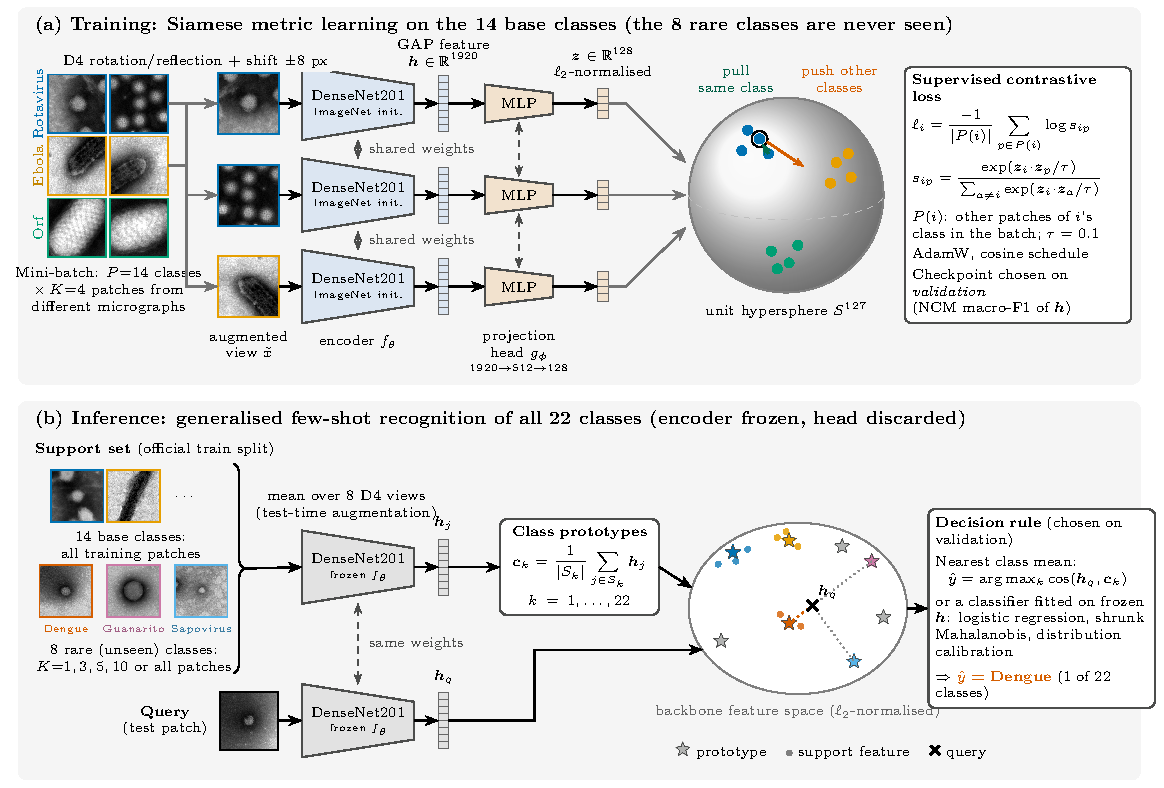
\includegraphics[width=\textwidth]{figures/architecture.pdf}
\caption{Overview of the method. (a) Training: patches of the 14 base classes pass through one DenseNet201 encoder with shared weights (drawn as parallel Siamese branches); a projection head maps the pooled feature $\bm{h}$ to a unit-norm embedding $\bm{z}$, and the supervised contrastive loss pulls together patches of the same virus and pushes apart patches of different viruses. (b) Inference: the head is discarded and the frozen encoder embeds the support patches of all 22 classes, including the eight rare classes never used for training, into class prototypes; a test patch is assigned by nearest class mean or by a classifier fitted on the frozen features, chosen on the validation split. Example patches are from the TEM virus dataset \cite{MS21data} (CC BY 4.0).}
\label{fig:arch}
\end{figure}

The encoder (Fig.~\ref{fig:arch}a) is an ImageNet-pretrained DenseNet201 \cite{Hua17,Den09}. Global average pooling gives a 1,920-dimensional \emph{backbone feature}; a projection head (1,920$\to$512$\to$128, L2-normalised) produces the embedding used by the loss. All patches pass through the same weights, so similarities are computed in one shared space. The network was trained with the supervised contrastive loss \cite{Kho20} (temperature 0.1) on batches of 14 classes $\times$ 4 patches, drawing the patches of a class from different micrographs where possible. Augmentation used the eight exact rotations and reflections of the square and translations of up to $\pm$8 pixels, which preserve physical scale. We used AdamW \cite{LH19} (learning rates $5\times10^{-5}$ for the backbone and $5\times10^{-4}$ for the head, weight decay $10^{-4}$, cosine schedule, at most 40 epochs). The checkpoint with the highest validation macro-F1 of nearest-prototype classification over the base classes was kept. The rare classes were never seen during training or model selection.

Pilot experiments in which four base classes were withheld from training showed that the backbone feature transfers to unseen classes whereas the 128-dimensional head does not (\ref{app:pilots}). We therefore fixed the backbone feature as the representation for all experiments before evaluating the main models.

\subsection{Baselines}
\label{sec:baselines}

\textbf{B1} re-implements the best benchmark model \cite{MS21} from its published configuration and code: DenseNet201, two fully connected layers of 1,024 units with dropout 0.3, and a 14-way softmax, trained with cross-entropy on the augmented training set (Adam, learning rate $10^{-5}$, batch size 12, 50 epochs, best validation accuracy). B1 and the Siamese encoder were each trained with \NSiamSeeds\ seeds. B1's pooled DenseNet201 features also serve as an alternative backbone in every few-shot experiment, which isolates the effect of the training objective. \textbf{B2}, a DenseNet201 with a linear head trained with class-balanced sampling on all 22 classes, sees the rare classes during training and is reported only as a fully supervised reference. Two loss ablations were trained once: batch-hard triplet loss \cite{Her17} and SupCon plus an auxiliary cosine-classifier term \cite{Che19}.

\subsection{Evaluation protocols}
\label{sec:protocols}

All results are on the official test split, with each patch represented by the mean over its eight rotations and reflections, computed with \InferenceMode\ inference. \emph{Closed set (14 classes):} nearest class mean with cosine similarity, prototypes from all training patches; B1 uses its softmax. \emph{GFSL (22 classes; Fig.~\ref{fig:arch}b):} prototypes for all classes from the training split; the 2,057 test patches are classified among all 22 classes. We report accuracy, macro-F1, base-class accuracy and rare-class mean per-class accuracy; the last is preferred to pooled accuracy because rare test sets range from 7 to 44 patches. \emph{K-shot GFSL:} as GFSL, but each rare class receives only $K\in\{1,3,5,10\}$ training patches from different micrographs (\KshotDraws\ random draws); base classes keep all training patches. Episode and unknown-virus detection results are given in \ref{app:extra}.

\subsection{Classifiers on frozen features}
\label{sec:classifiers}

To test whether rare-class errors stem from the representation or from the decision rule, we fitted four classifiers on the frozen backbone features of every checkpoint, without modifying the encoder:
nearest class mean (NCM);
L2-regularised logistic regression (LR) with class-balanced weights \cite{Tia20};
a Mahalanobis classifier with class covariances shrunk towards the pooled covariance in a 64--256-dimensional principal-component space, following Simple CNAPS \cite{Bat20}; and
distribution calibration (DC), which samples synthetic features for each rare class from the statistics of its nearest base classes \cite{Yan21}.
Each classifier was fitted on the training split and its hyper-parameters chosen by 22-class validation macro-F1; the chosen setting was applied once to the test split. Before seeing any test result we fixed the rule that the classifier with the highest validation macro-F1 is the one reported as the improvement; all four are reported. In a separability diagnostic, a binary LR was trained on the training patches of each of eight confusable pairs and evaluated on their validation patches.

\subsection{Statistics}
\label{sec:stats}

Confidence intervals (95\,\%) come from a stratified micrograph-level cluster bootstrap that resamples micrographs within classes \cite{ET93}. Paired comparisons on identical test patches use a paired cluster bootstrap of the difference in accuracy and macro-F1, together with an exact McNemar test \cite{McN47}. McNemar treats patches as independent and is anti-conservative when patches share micrographs, so conclusions rest on the cluster bootstrap. Siamese--B1 comparisons are made for all $3\times3$ seed pairs, and K-shot comparisons are paired over identical support draws. Values over seeds are mean $\pm$ standard deviation.

\subsection{Implementation}
\label{sec:impl}

Experiments used PyTorch 2.11 and scikit-learn on one NVIDIA RTX 3060 (12\,GB). The analysis code was written with the assistance of an AI tool (Claude, Anthropic) and was checked with 23 automated tests, including comparisons of the loss functions and evaluation metrics against independent reference implementations. Training took 19--28\,min per Siamese seed and about 134\,min for B1.

%% ======================================================================
\section{Results}
\label{sec:results}

\subsection{14-class benchmark}

The Siamese encoder matched B1 (Table~\ref{tab:closed}). Over the \SeedClosedN\ Siamese--B1 seed pairs, the paired accuracy difference ranged from \SeedClosedRange\ points; it favoured the Siamese encoder in \SeedClosedNPos\ pairs, but its cluster CI excluded zero in \SeedClosedNSig\ of \SeedClosedN\ (macro-F1: \SeedClosedFOneRange, CI excluding zero in \SeedClosedFOneNSig\ of \SeedClosedN). For seed 0 versus seed 0, the accuracy difference was \CmpFeatDiff\ points (95\,\% CI \CmpFeatCI; McNemar \CmpFeatMcN\ discordant patches, $p=\CmpFeatMcP$). Every seed of both models exceeded the published 93.1\,\%; because test-time augmentation and implementation details differ, B1 rather than the published figure is the fair comparator. The 128-dimensional head scored slightly higher on the base classes (\SiamHeadClosedAcc\,\%), but it was not the pre-specified representation, its CI against B1 (seed 0) includes zero (\CmpHeadCI), and it fails on unseen classes (Section~\ref{sec:res-gfsl}).

\begin{table}[t]
\centering\footnotesize
\caption{14-class official test split (1,900 patches, 206 micrographs). Macro-averaged precision, sensitivity (recall) and specificity; mean $\pm$ SD over seeds. $^{a}$Without test-time augmentation.}
\label{tab:closed}
\resizebox{\textwidth}{!}{%
\begin{tabular}{lrrrrrr}
\toprule
Model & Acc.\ (\%) & Macro-F1 & Prec. & Sens. & Spec. & Micrograph acc.\ (\%) \\
\midrule
\TabClosedRows
\bottomrule
\end{tabular}}
\end{table}

\subsection{22-class generalised few-shot recognition}
\label{sec:res-gfsl}

With nearest-prototype classification over all 22 classes, Siamese and B1 features reached the same macro-F1 (\SiamGfslFOne\ vs \BOneGfslFOne; Table~\ref{tab:gfsl}). Siamese features were more accurate overall (\SiamGfslAcc\,\% vs \BOneGfslAcc\,\%), mainly through the base classes (\SiamGfslBase\,\% vs \BOneGfslBase\,\%), whereas B1 features recognised the rare classes slightly better (rare mean-class accuracy \BOneGfslRare\,\% vs \SiamGfslRare\,\%). Over the \SeedNcmN\ seed pairs the paired accuracy difference ranged from \SeedNcmRange\ points, with a cluster CI excluding zero in \SeedNcmNSig\ of \SeedNcmN; for seed 0 the McNemar test gave $p=\CmpGfslMcP$ although the cluster CI \CmpGfslCI\ includes zero, illustrating its anti-conservatism. The 128-dimensional head collapsed on the rare classes (rare mean-class accuracy \HeadRareMin--\HeadRareMax\,\%). A large gap remained to B2, which was trained on the rare classes. Errors concentrated in a few rare viruses: \DengueToSapMin--\DengueToSapMax\ of the \DengueTest\ Dengue test patches were assigned to Sapovirus in every seed.

\begin{table}[t]
\centering\footnotesize
\caption{22-class GFSL on the official test split (2,057 patches, 252 micrographs) with nearest-class-mean classification; rare classes enter only as prototypes.}
\label{tab:gfsl}
\resizebox{\textwidth}{!}{%
\begin{tabular}{lrrrr}
\toprule
Features & Acc.\ (\%) & Macro-F1 & Base acc.\ (\%) & Rare mean-class acc.\ (\%) \\
\midrule
\TabGfslRows
\bottomrule
\end{tabular}}
\end{table}

\subsection{Rare classes are separable}

Every confusable pair was close to linearly separable in the learned features (validation AUROC $\geq$ \SepAucMin; Table~\ref{tab:sep}), yet the two-class nearest-mean rule was far below the linear boundary for several pairs. For Sapovirus versus Astrovirus it was near chance (\SapAstNcmMin--\SapAstNcmMax) while LR reached \SapAstLrMin--\SapAstLrMax. The information needed to recognise the rare viruses is therefore present in the representation but not exploited by isotropic distance to a class mean. The rare-class validation sets are small (10--16 patches), so these values are indicative.

\begin{table}[t]
\centering\footnotesize
\caption{Pairwise separability on the validation split (binary LR trained on training patches). Values are means over the three seeds of each encoder.}
\label{tab:sep}
\resizebox{\textwidth}{!}{%
\begin{tabular}{lrrrrr}
\toprule
 & \multicolumn{3}{c}{Siamese features} & B1 features & \\
\cmidrule(lr){2-4}
Pair & AUROC & LR acc. & NCM acc. & AUROC & Val.\ patches \\
\midrule
\TabSepRows
\bottomrule
\end{tabular}}
\end{table}

\subsection{Classifiers on frozen features}

The pre-declared rule selected LR for \LrWinsN\ of the \NCheckpoints\ checkpoints, including all three Siamese seeds (exception: \LrWinExceptions; Table~\ref{tab:clf}). For the Siamese encoder, LR raised 22-class macro-F1 from \SiamNcmFOne\ to \SiamLrFOne\ and accuracy from \SiamNcmAcc\,\% to \SiamLrAcc\,\%, while base-class accuracy also rose (\SiamNcmBase\ to \SiamLrBase\,\%). The paired macro-F1 gain of LR over NCM ranged from \PairLrNcmAllRange\ and its cluster CI excluded zero for \PairLrNcmAllSig\ of the \PairLrNcmAllN\ checkpoints. Dengue F1 rose from \WeakDengueNcm\ to \WeakDengueLr, Sapovirus from \WeakSapovirusNcm\ to \WeakSapovirusLr\ and Guanarito from \WeakGuanaritoNcm\ to \WeakGuanaritoLr\ (Appendix Table~\ref{tab:weak}). The Mahalanobis classifier reached a similar macro-F1 (\SiamMahaFOne), but its validation optimum was nearly flat across settings (smallest gap between the best two settings \MahaMinValGap), so its test result depends on near-ties; we report it as secondary.

With full rare-class training data the Siamese objective gave no advantage: LR on B1 features reached macro-F1 \BOneLrFOne\ versus \SiamLrFOne\ for Siamese features. Across the \PairSiamBOneLrN\ seed pairs the paired macro-F1 difference (Siamese minus B1) ranged from \PairSiamBOneLrRange, with a CI excluding zero in \PairSiamBOneLrNSig\ of the \PairSiamBOneLrN\ pairs (\PairSiamBOneLrSigDir).

Classifiers that estimate more parameters needed more data. With one example per rare class, LR fell to \SiamLrKOne\,\% rare mean-class accuracy against \SiamNcmKOne\,\% for NCM, whereas DC improved on NCM (\SiamDcKOne\,\%; paired gain \PairDcRange\ points, significant for \PairDcNSig\ of \PairDcN\ Siamese and B1 checkpoints). With DC, Siamese and B1 features performed similarly at one shot (\SiamDcKOne\,\% vs \BOneDcKOne\,\%).

\begin{table}[t]
\centering\footnotesize
\caption{22-class GFSL on the official test split with classifiers on frozen backbone features; hyper-parameters selected on validation. $K=1$, $K=5$: rare mean-class accuracy with only $K$ training patches per rare class (\PairKOneDraws\ draws). Superscripts: number of seeds for which the classifier had the highest validation macro-F1.}
\label{tab:clf}
\resizebox{\textwidth}{!}{%
\begin{tabular}{llrrrrrr}
\toprule
Features & Classifier & Val.\ F1 & Acc.\ (\%) & Macro-F1 & Rare (\%) & $K{=}1$ (\%) & $K{=}5$ (\%) \\
\midrule
\TabClassifierRows
\bottomrule
\end{tabular}}
\end{table}

\subsection{Few-shot regime}

With one training patch per rare virus, Siamese features gave higher rare-class accuracy than B1 features (\KshotSiamOne\,\% vs \KshotBOneOne\,\%; Table~\ref{tab:kshot}); paired over identical support draws, the difference ranged from \PairKOneRange\ points and was significant for \PairKOneNSig\ of \PairKOneN\ Siamese--B1 pairs. From three examples onwards B1 features were equal or better.

\begin{table}[t]
\centering\footnotesize
\caption{K-shot GFSL with nearest class mean: rare-class mean accuracy (\%) when each rare class has $K$ training patches (\KshotDraws\ draws).}
\label{tab:kshot}
\begin{tabular}{rrr}
\toprule
$K$ & Siamese features & B1 features \\
\midrule
\TabKshotRows
\bottomrule
\end{tabular}
\end{table}

%% ======================================================================
\section{Discussion}
\label{sec:discussion}

Under an identical, leakage-audited protocol, a Siamese supervised-contrastive encoder with a nearest-prototype classifier matched a re-implementation of the strongest published benchmark model on the 14 base classes, and its features allow new virus classes to be added without retraining. In the most data-scarce setting, a single reference patch per new virus classified by nearest prototype, it recognised rare viruses better than features learned with cross-entropy, consistently across all seed pairs. This is the regime that motivates few-shot learning for diagnostic TEM: the first image of an emerging virus can be added as a prototype immediately.

The advantage did not persist with three or more examples, in rare-class-only episodes, when distribution calibration was used, or once a linear classifier was fitted on all available rare-class data; with nearest-prototype classification over all 22 classes the two feature sets also reached the same macro-F1. This agrees with the finding that the quality of the embedding, rather than the metric-learning objective, dominates few-shot performance \cite{Che19,Tia20}, and it shows that claims of superiority for metric-learning approaches on this dataset should be tested against an identically evaluated classification baseline.

The most actionable result concerns the rare classes that previous 22-class work did not analyse. Dengue, Sapovirus, Guanarito and LCM were poorly recognised by prototype classification although they are nearly linearly separable from their confusers in the same feature space. Distance to a class mean ignores differences in class spread, which is plausible for rare classes whose few micrographs differ in staining and particle density. A validation-selected logistic regression recovered much of the gap to the fully supervised reference B2 (macro-F1 \SiamLrFOne\ vs \CeFOne) without retraining the encoder. It needs enough examples, however: with one to five examples per class, nearest-mean or distribution calibration should be preferred.

Published 22-class results train on all classes and use different or unreported splits \cite{U24,H26}, so they are not directly comparable with ours; B2, trained on all classes with our pipeline, reached \CeAcc\,\% accuracy on the official split.

\textbf{Limitations.} The rare classes have 2--8 test micrographs each, so per-class F1 for Sapovirus (8 patches) and Guanarito (7 patches) is highly uncertain. The ablations were trained once. Hyper-parameters of the frozen-feature classifiers were chosen on small rare-class validation sets, which adds selection variance, as the Mahalanobis results show. We studied one backbone and one dataset, and unknown-virus detection (\ref{app:extra}) is not yet adequate for deployment.

%% ======================================================================
\section{Conclusions}

We present the first generalised few-shot evaluation of all 22 classes of the public TEM virus dataset on its official split, with the rare classes never used for training. A Siamese metric-learning encoder matches a strong re-implemented classifier on the benchmark and, with nearest-prototype classification, recognises rare viruses better when only one reference patch is available, but not with more examples. Most of the attainable improvement on rare viruses comes from replacing nearest-prototype classification with a validation-selected linear classifier on frozen features, for either training objective. The protocol, code and per-patch predictions are released for future comparisons.

%% ======================================================================
\section*{Declaration of competing interests}
The author declares no known competing financial interests or personal relationships that could have appeared to influence the work reported in this paper.

\section*{Funding}
This research did not receive any specific grant from funding agencies in the public, commercial, or not-for-profit sectors.

\section*{CRediT authorship contribution statement}
\textbf{S. M. Mahbub Uddin Ahmed:} Conceptualization, Methodology, Software, Validation, Formal analysis, Investigation, Data curation, Visualization, Writing -- original draft, Writing -- review \& editing.

\section*{Data and code availability}
The TEM virus dataset is publicly available \cite{MS21data}. Code, configurations, training logs, evaluation outputs and per-patch predictions are available at \url{https://github.com/hrid0yyy/tem-virus-siamese-fewshot} \textcolor{red}{[TODO before submission: repository is still private -- make it public or change this URL]}; trained checkpoints are available as release assets.

\section*{Declaration of generative AI and AI-assisted technologies in the manuscript preparation process}
During the preparation of this work the author used Claude (Anthropic) in order to assist with writing the analysis code and with drafting and editing the manuscript text. After using this tool, the author reviewed and edited the content as needed and takes full responsibility for the content of the published article.

%% ======================================================================
\appendix

\section{Pilot experiments}
\label{app:pilots}

Four base classes were withheld from encoder training (F2: Astrovirus, Influenza, Papilloma, Rotavirus; F3: Marburg, Orf, Adenovirus, CCHF) and used as unseen classes, with micrograph-disjoint episodes (600 episodes, 15 queries per class). Without training, ImageNet features reached only \PilotFrozenNcm\,\% nearest-mean accuracy on the 14 classes (\PilotFrozenProbe\,\% with a linear probe). After training, the backbone feature transferred to the unseen classes, whereas the 128-dimensional head did not; in the F3 GFSL test head accuracy on the unseen classes was \PilotHeadUnseen\,\% (Table~\ref{tab:pilots}).

\begin{table}[h]
\centering\footnotesize
\caption{Pilot experiments (accuracy in \%, or harmonic mean of base and unseen accuracy).}
\label{tab:pilots}
\resizebox{\textwidth}{!}{%
\begin{tabular}{lrrr}
\toprule
Experiment & Frozen ImageNet & Trained, backbone feature & Trained, 128-d head \\
\midrule
\TabPilotRows
\bottomrule
\end{tabular}}
\end{table}

\section{Additional results}
\label{app:extra}

\begin{table}[h]
\centering\footnotesize
\caption{Test F1 of the weakest rare classes. Test patches: \WeakSupport.}
\label{tab:weak}
\resizebox{\textwidth}{!}{%
\begin{tabular}{lrrrrr}
\toprule
Features, classifier & Dengue & Sapovirus & Guanarito & LCM & Machupo \\
\midrule
\TabWeakRows
\bottomrule
\end{tabular}}
\end{table}

\begin{table}[h]
\centering\footnotesize
\caption{8-way episodes over the rare classes (micrograph-disjoint support and query, 600 episodes) and unknown-virus detection (rare-class test patches as unknown; score = maximum cosine similarity to the 14 base prototypes).}
\label{tab:episodes}
\resizebox{\textwidth}{!}{%
\begin{tabular}{lrrrr}
\toprule
Features & 1-shot (\%) & 5-shot (\%) & AUROC & FPR at 95\,\% TPR (\%) \\
\midrule
\TabEpisodesRows
\bottomrule
\end{tabular}}
\end{table}

\bibliographystyle{elsarticle-num}
\bibliography{references}

\end{document}
